\documentclass[conference]{IEEEtran}
\IEEEoverridecommandlockouts
% The preceding line is only needed to identify funding in the first footnote. If that is unneeded, please comment it out.
\usepackage{cite}
\usepackage{amsmath,amssymb,amsfonts}
\usepackage{algorithmic}
\usepackage{graphicx}
\usepackage{textcomp}
\usepackage{xcolor}
\def\BibTeX{{\rm B\kern-.05em{\sc i\kern-.025em b}\kern-.08em
    T\kern-.1667em\lower.7ex\hbox{E}\kern-.125emX}}
%\usepackage{hyperref}

\usepackage{listings} 

\usepackage{amsmath}

\newtheorem{program}{Program}



\begin{document}

\title{Introduction to Static \& Dynamic Library\\
%{\footnotesize \textsuperscript{*}Note: Sub-titles are not captured in Xplore and
%should not be used}
\thanks{The author is with 5G Lab, IISc Bangalore. Email: kprasannakumar.iith@gmail.com, prasannakk@iisc.ac.in}
}

\author{K. Prasanna Kumar}

\maketitle

\tableofcontents


\begin{abstract}
This module explains how to create user defined static and dynamic libraries using C or C++ Programming in Linux Operating System.
\end{abstract}

%\begin{IEEEkeywords}
%Share Library 
%\end{IEEEkeywords}

\section{Introduction}
\begin{itemize}
\item \textbf{Function :} Group of pre-compiled codes.
\item \textbf{Library :} Package of functions, to avoid repetition of codes.
\item There are two type of libraries
\begin{enumerate}
\item Static Library
\item Dynamic Library
\end{enumerate}
\item Library is not an executable. It is used either at compile time or run time.
\end{itemize}
\section{Executable File}
\begin{figure}[h!]
\centering
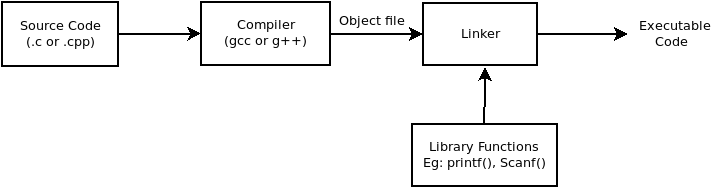
\includegraphics[scale=0.32]{img/exe_block.png}
\label{Steps to Create Executable File}
\caption{Steps to Create Executable File}
\end{figure}
\program
Create an executable for the following C program \textbf{"Finding the largest number in the array"}
\lstinputlisting[frame=single]{code/lrg_ele_ary.c}

\subsection*{Commands to build Executable}
\begin{itemize}
\item Compile the code using following command.
\begin{lstlisting}
gcc -c lrg_array.c -o larg_arry.o
\end{lstlisting}

\item Generating an executable by linking to libraries
\begin{lstlisting}
gcc larg_arry.o -o larg_arry
\end{lstlisting}

\item Run the executable 
\begin{lstlisting}
./larg_arry
\end{lstlisting}

\end{itemize}

\program
Generating samples of sine signal with sample time $T_s$ = 0.1 in the range $[0, 2\pi]$ 
\lstinputlisting[frame=single]{code/sine_sig.c}

\subsection*{Commands to build Executable}
\begin{itemize}
\item
Compile the code using following command.
\begin{lstlisting}
gcc -c sine_sig.c -o sine_sig.o
\end{lstlisting}
\item 
Generating an executable by linking to libraries
\begin{lstlisting}
gcc sine_sig.o -lm -o sine_sig
\end{lstlisting}
\textbf{"-lm"} is for linking math library.
\item 
Run the executable 
\begin{lstlisting}
./sine_sig
\end{lstlisting}

\end{itemize}

\section{Static Library}
\program
Program file with function definitions of arithmetic operations
\lstinputlisting[frame=single]{code/arthematic.c }

\program
Program file with function definitions of Bit-wise operations
\lstinputlisting[frame=single]{code/logic.c }

\program
Header file
\lstinputlisting[frame=single]{code/alu.h }

\program 
main file
\lstinputlisting[frame=single]{code/alu.c }

\subsection*{Commands to build static lib}
\begin{itemize}
\item Compilation of Source codes except the main to generate the object files
\begin{lstlisting}
gcc -c arthematic.c -o arthematic.o
gcc -c logic.c -o logic.o
\end{lstlisting}
\item Create a static library using above created objects files by using the following command
\begin{lstlisting}
ar rcs libalu.a arthematic.o logic.o
\end{lstlisting}
\item Compilation of main program generate object file
\begin{lstlisting}
gcc -c alu.c -o alu.o
\end{lstlisting}
\item Linking static library main program object file to create executable 
\begin{lstlisting}
gcc alu.o -L. libalu.a -o alu
\end{lstlisting}
Extension to static library is ".a"
\item Running executable
\begin{lstlisting}
./alu
\end{lstlisting}
\end{itemize}
\section{Dynamic Library}
Programs in used in building static library can be used for building dynamic library. Dynamic library is also know as shared library
\subsection*{Commands to build dynamic lib}
\begin{itemize}
\item Compilation of Source codes except the main to generate the object files
\begin{lstlisting}
gcc -c arthematic.c logic.c -fpic
\end{lstlisting}
"-fpic " will create object files for all the sources codes mentioned in the command.
\item Combining all the object files to create shared library
\begin{lstlisting}
gcc *.o -shared -o libpraalu.so
\end{lstlisting}
Extension to shared library is ".so"
\item Copy the shared library generated to "/usr/lib"
\begin{lstlisting}
sudo cp /usr/lib/libpraalu.so
\end{lstlisting}
\item Compilation of main program generate object file
\begin{lstlisting}
gcc -c alu.c -o alu.o
\end{lstlisting}
\item Linking dynamic library main program object file to create executable 
\begin{lstlisting}
gcc alu.o -L. -libpraalu.so -o alu
\end{lstlisting}

 or
 
\begin{lstlisting}
gcc alu.o -L. -lpraalu.so -o alu
\end{lstlisting}
\item Running executable
\begin{lstlisting}
./alu
\end{lstlisting}
\end{itemize}

\begin{thebibliography}{00}
\bibitem{b1} iFocus Institute, YOUTUBE CHANEL
%\url{https://www.youtube.com/channel/UCs4fiPaL4_B_xYx9FM_Xekw}
\bibitem{b2} Dia, Software used to build flowcharts 


\end{thebibliography}


\end{document}
